\documentclass[a4paper,10pt]{article}
\usepackage{graphicx}
\usepackage{listings}
\usepackage{hyperref}

% Title Page
\title{Homework 1: Harris-affine corners}
\author{Francis Vo}


\begin{document}
\maketitle

\begin{figure}[h!]
% \begin{table}[h!]
    \begin{center}
		\begin{tabular}{ | c | c | c | c | }
		\hline
		Threshold & bike\_001 & bike\_002 & bike\_003 \\ \hline
		100 & 
\includegraphics[width=0.27\textwidth]{bike_001_100.png} & 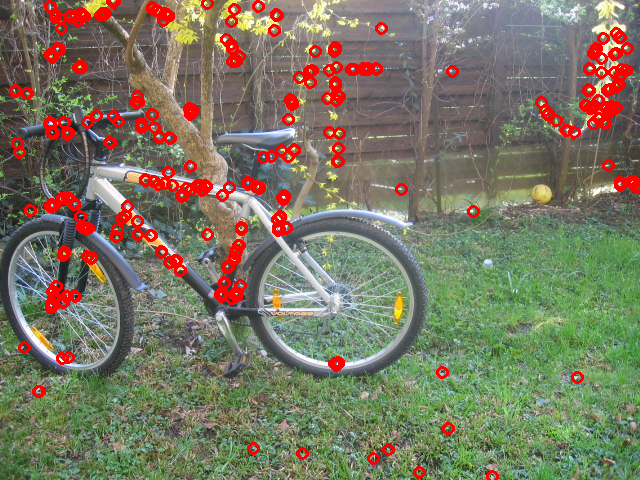
\includegraphics[width=0.27\textwidth]{bike_002_100.png} & 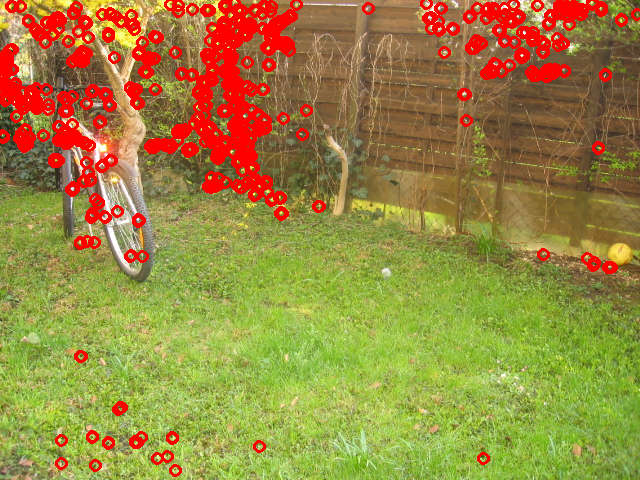
\includegraphics[width=0.27\textwidth]{bike_003_100.png} \\ \hline
		150 & 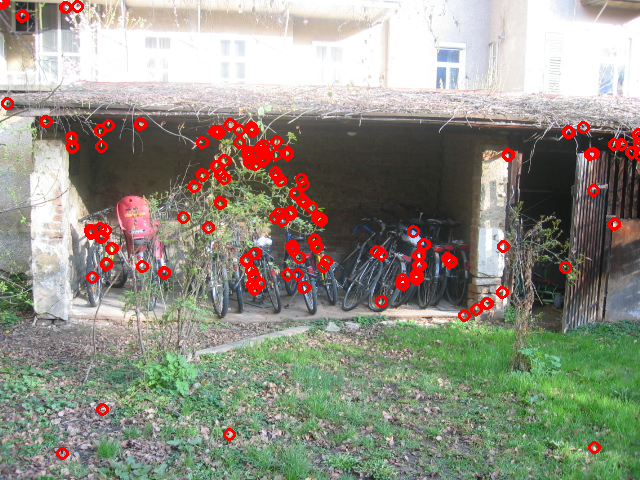
\includegraphics[width=0.27\textwidth]{bike_001_150.png} & 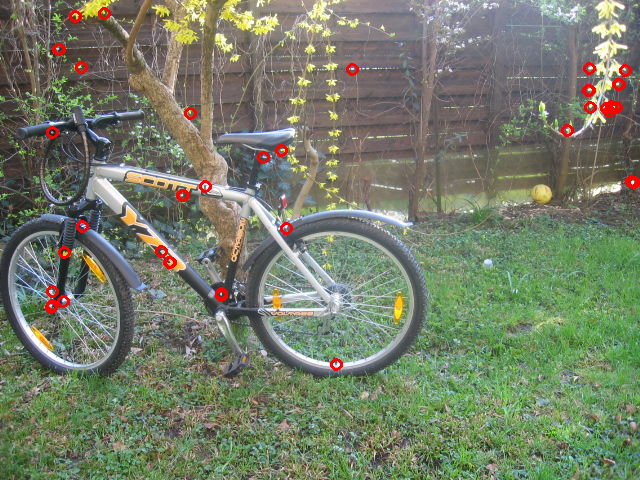
\includegraphics[width=0.27\textwidth]{bike_002_150.png} & 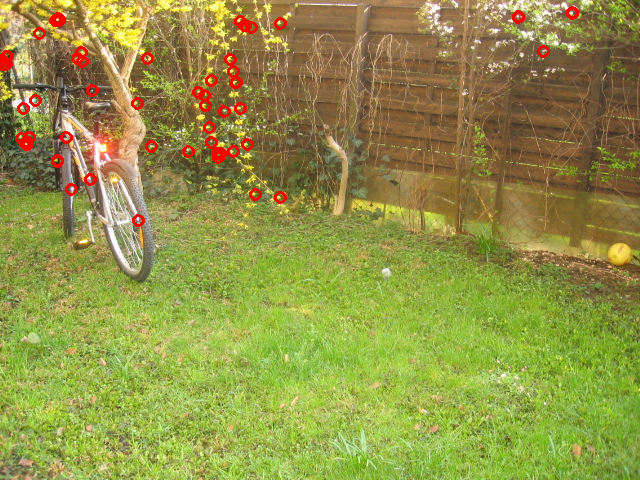
\includegraphics[width=0.27\textwidth]{bike_003_150.png} \\ \hline
		200 & 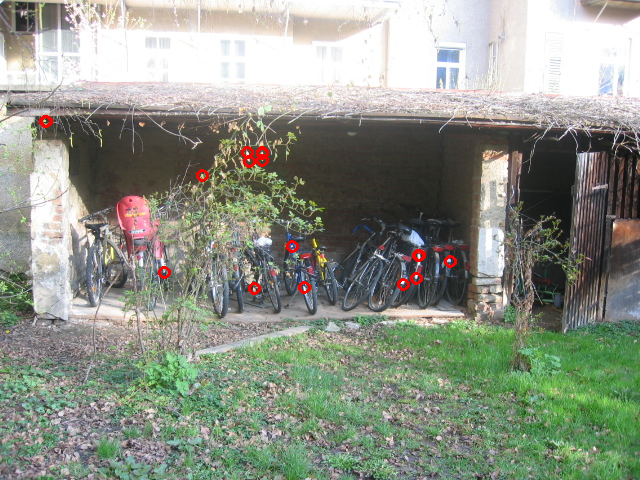
\includegraphics[width=0.27\textwidth]{bike_001_200.png} & 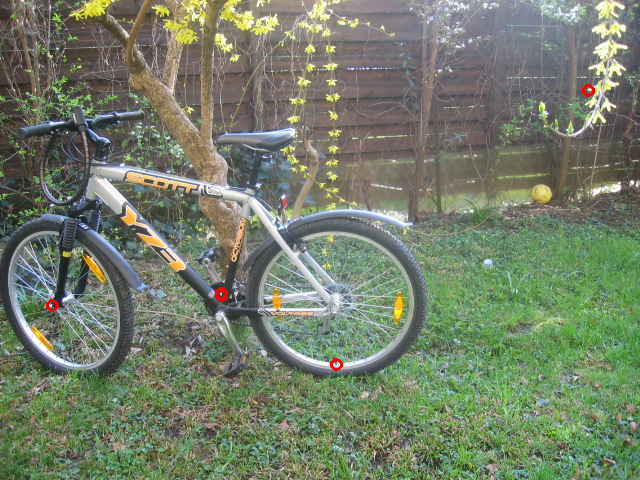
\includegraphics[width=0.27\textwidth]{bike_002_200.png} & 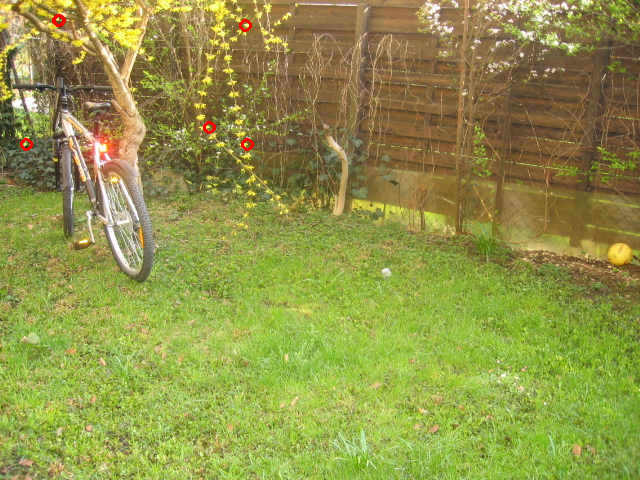
\includegraphics[width=0.27\textwidth]{bike_003_200.png} \\ \hline

		\end{tabular}
	\end{center}
% \end{table}
\caption{Harris-affine corners superimposed on example images}
\end{figure}

% Table 1: the mean descriptor vector of each cluster, i.e., the 300 cluster centers, for SIFT descriptors.
\begin{table}[h!]
	\begin{center}
		\begin{tabular}{ | c | c | c | c | }
		
		\end{tabular}
	\end{center}
\caption{the mean descriptor vector of each cluster, i.e., the 300 cluster centers, for SIFT descriptors}
\end{table}

\begin{table}[h!]
	\begin{center}
		\begin{tabular}{ | c | c | c | c | }
		
		\end{tabular}
	\end{center}
\caption{the mean descriptor vector of each cluster, i.e., the 300 cluster centers, for HOG descriptors}
\end{table}

\begin{figure}[h!]

\caption{image patches used for computing SIFT clusters}
\end{figure}

\begin{figure}[h!]

\caption{image patches used for computing HOG clusters}
\end{figure}

% Show in Figure 2 and Figure 3 two tables of image patches used for computing SIFT and
% HOG clusters, respectively, as illustrated below. Each table should have 10 rows and 10 columns.
% The rows correspond to the 10 largest clusters you computed using the K-means algorithm. The
% 10 columns of one row should contain 10 image patches that are the closest to the cluster center
% of that row. The image patches are image areas around the Harris-affine corners that are used
% to compute SIFT or HOG descriptors. The distance between image patches is computed as the
% Euclidean distance between the associated SIFT or HOG descriptors.

\section{Source Code}
The original harris detector code was from \url{http://docs.opencv.org/doc/tutorials/features2d/trackingmotion/harris_detector/harris_detector.html} written by the Opencv team.

\lstinputlisting{cornerHarris.cpp}

\end{document}          
